\documentclass[aspectratio=169, 10pt]{beamer}

% --- 1. CẤU HÌNH GÓI VÀ NGÔN NGỮ ---
\usepackage[utf8]{vietnam}
\usepackage{amsmath, amssymb, amsthm}
\usepackage{graphicx}
\usepackage{hyperref}
\usepackage{wrapfig}
\usepackage{multicol}
\usepackage{adjustbox}

% --- 2. CẤU HÌNH ĐỒ HỌA (TIKZ & PGFPLOTS) ---
\usepackage{tikz}
\usepackage{pgfplots}
\pgfplotsset{compat=1.17}
\usetikzlibrary{calc, shapes.geometric, arrows.meta, 3d, intersections, patterns, backgrounds}
\usepgfplotslibrary{fillbetween}

% --- 3. THEME & MÀU SẮC & HIỆU ỨNG ---
\usetheme{Madrid}
\usecolortheme{default}
\definecolor{UETBlue}{RGB}{0, 64, 122}
\setbeamercolor{structure}{fg=UETBlue}
\setbeamercolor{palette primary}{bg=UETBlue, fg=white}
\setbeamercolor{frametitle}{bg=UETBlue, fg=white}

% [QUAN TRỌNG] Cấu hình để nội dung chưa hiện sẽ mờ đi chứ không ẩn hẳn
\setbeamercovered{transparent}

% --- 4. THÔNG TIN BÀI GIẢNG ---
\title[Phương pháp Vỏ trụ]{PHƯƠNG PHÁP VỎ TRỤ (CYLINDRICAL SHELLS)}
\subtitle{Chi tiết Lý thuyết và Bài tập (Stewart Calculus 5.3)}
\author[Nhóm 7 - IS5]{Nhóm 7 - IS5 \\ Khoa Công nghệ Thông tin}
\institute[VNU-UET]{
    \textbf{ĐẠI HỌC CÔNG NGHỆ - ĐHQGHN}\\
    (VNU University of Engineering and Technology)
}
\date{\today}

\begin{document}

% Slide 0: Title
\begin{frame}
    \transdissolve % Hiệu ứng tan biến nhẹ khi vào bài
    \titlepage
\end{frame}

% Slide 0b: Mục lục
\begin{frame}{Nội dung trình bày}
    \tableofcontents
\end{frame}

% =========================================================
% PHẦN 1: LÝ THUYẾT
% =========================================================
\section{Xây dựng Công thức (Lý thuyết)}

% Slide 1: Đặt vấn đề
\begin{frame}{1. Đặt vấn đề: Tại sao cần Phương pháp Vỏ trụ?}
    \begin{columns}
        \column{0.65\textwidth}
        \small 
        Xét bài toán tìm thể tích vật thể tròn xoay khi quay miền $y = 2x^2 - x^3$ và $y=0$ quanh trục $y$.
        % [HIỆU ỨNG] <+-> nghĩa là hiện từng dòng một
        \begin{itemize}[<+->]
            \item \textbf{Nếu dùng phương pháp Lát cắt (Washer):}
            \begin{itemize}
                \item Cắt vuông góc trục $y$ $\Rightarrow$ Phải tích phân theo $dy$.
                \item Cần tìm hàm ngược $x=g(y)$ từ $y = 2x^2 - x^3$.
                \item \textbf{Khó khăn:} Đây là phương trình bậc 3, rất khó giải $x$ theo $y$.
            \end{itemize}
            \item \textbf{Giải pháp:} Cần phương pháp tích phân theo $dx$ nhưng quay quanh trục $y$. $\Rightarrow$ \textbf{Phương pháp Vỏ trụ}.
        \end{itemize}

        \column{0.35\textwidth}
        \centering
        \resizebox{\linewidth}{!}{
            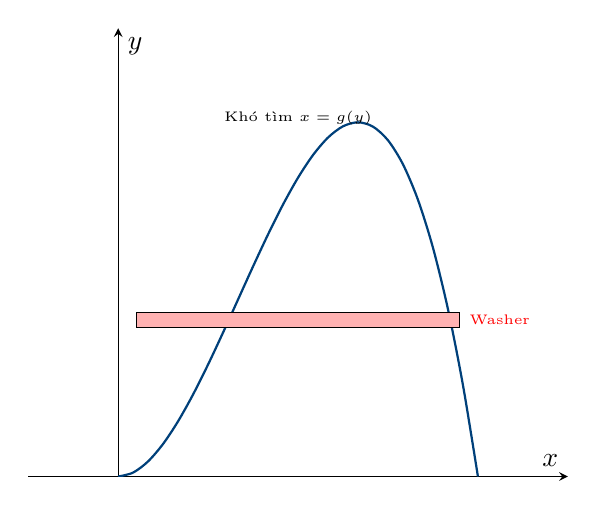
\begin{tikzpicture}
                \begin{axis}[axis lines=middle, xtick=\empty, ytick=\empty, xlabel=$x$, ylabel=$y$, xmin=-0.5, xmax=2.5, ymin=0, ymax=1.5]
                     \addplot[thick, UETBlue, domain=0:2, smooth] {2*x^2 - x^3};
                     \node at (axis cs:1, 1.2) {\tiny Khó tìm $x=g(y)$};
                     \draw[fill=red!30] (axis cs:0.1, 0.5) rectangle (axis cs:1.9, 0.55);
                     \node[right, red] at (axis cs:1.9, 0.525) {\tiny Washer};
                \end{axis}
            \end{tikzpicture}
        }
    \end{columns}
\end{frame}

% Slide 2: Chứng minh hình học
\begin{frame}{2. Xây dựng công thức: Từ hình học sơ cấp}
    \small
    Xét vỏ trụ bán kính trong $r_1$, bán kính ngoài $r_2$, chiều cao $h$.
    \begin{columns}
        \column{0.6\textwidth}
        Thể tích $V$ là hiệu thể tích trụ ngoài và trụ trong:
        \begin{align*}
            V &= \pi r_2^2 h - \pi r_1^2 h = \pi h (r_2^2 - r_1^2) \\
              &= \pi h (r_2 + r_1)(r_2 - r_1) \\
              \onslide<2->{&= 2\pi h \cdot \underbrace{\frac{r_2 + r_1}{2}}_{r_{\text{tb}}} \cdot \underbrace{(r_2 - r_1)}_{\Delta r}}
        \end{align*}
        
        % [HIỆU ỨNG] Pause để dừng lại nhấn mạnh trước khi hiện công thức chốt
        \pause 
        
        \begin{alertblock}{Công thức xấp xỉ}
            \[ V \approx 2\pi r h \Delta r = (\text{Chu vi}) \cdot (\text{Cao}) \cdot (\text{Dày}) \]
        \end{alertblock}

        \column{0.4\textwidth}
        \centering
        \resizebox{0.8\linewidth}{!}{
            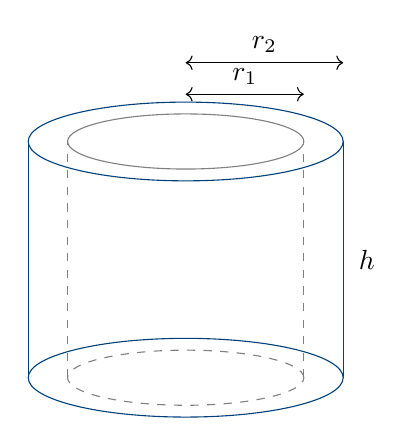
\begin{tikzpicture}
                \def\rTwo{2} \def\rOne{1.5} \def\h{3}
                \draw[UETBlue] (0,0) ellipse ({\rTwo} and 0.5);
                \draw[UETBlue] (-\rTwo,0) -- (-\rTwo,\h);
                \draw[UETBlue] (\rTwo,0) -- (\rTwo,\h);
                \draw[UETBlue] (0,\h) ellipse ({\rTwo} and 0.5);
                \draw[dashed, gray] (0,0) ellipse ({\rOne} and 0.35);
                \draw[gray] (0,\h) ellipse ({\rOne} and 0.35);
                \draw[dashed, gray] (-\rOne,0) -- (-\rOne,\h);
                \draw[dashed, gray] (\rOne,0) -- (\rOne,\h);
                \draw[<->] (0, \h+0.6) -- (\rOne, \h+0.6) node[midway, above] {$r_1$};
                \draw[<->] (0, \h+1.0) -- (\rTwo, \h+1.0) node[midway, above] {$r_2$};
                \node at (\rTwo+0.3, \h/2) {$h$};
            \end{tikzpicture}
        }
    \end{columns}
\end{frame}

% Slide 3: Tổng Riemann (Giữ nguyên hoặc thêm pause nhẹ)
\begin{frame}{3. Xây dựng tích phân (Tổng Riemann)}
    \begin{columns}
        \column{0.6\textwidth}
        \small
        Chia đoạn $[a, b]$ thành $n$ đoạn con $\Delta x$. Lấy mẫu $\overline{x}_i$.
        \begin{itemize}[<+->]
            \item Quay hình chữ nhật tại $\overline{x}_i$ quanh trục $y$ tạo thành vỏ trụ.
            \item Bán kính $r_i = \overline{x}_i$, Chiều cao $h_i = f(\overline{x}_i)$.
        \end{itemize}
        
        \onslide<3->{
            Tổng Riemann xấp xỉ thể tích:
            \[ V \approx \sum_{i=1}^{n} 2\pi \overline{x}_i f(\overline{x}_i) \Delta x \]
            Cho $n \to \infty$, ta được tích phân xác định.
        }

        \column{0.4\textwidth}
        \centering
        \resizebox{\linewidth}{!}{
             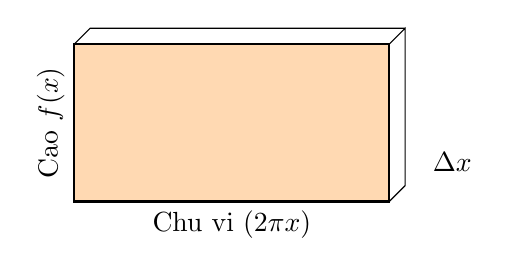
\begin{tikzpicture}
                % Hình hộp
                \fill[orange!30] (0,0) rectangle (4, 2);
                \draw[thick] (0,0) rectangle (4, 2);
                \node at (2, -0.3) {Chu vi ($2\pi x$)};
                \node[rotate=90] at (-0.3, 1) {Cao $f(x)$};
                \draw (4,0) -- (4.2,0.2) -- (4.2, 2.2) -- (4, 2);
                \draw (0,2) -- (0.2, 2.2) -- (4.2, 2.2);
                \node at (4.8, 0.5) {$\Delta x$};
            \end{tikzpicture}
        }
    \end{columns}
\end{frame}

% Slide 4: Công thức chính thức
\begin{frame}{4. Định lý và Công thức Ghi nhớ}
    \begin{block}{Định lý (Phương pháp Vỏ trụ)}
        Thể tích vật thể khi quay miền giới hạn bởi $y=f(x)$, $y=0$, $x=a$, $x=b$ ($0 \le a < b$) quanh trục $y$:
        \[ V = \int_{a}^{b} 2\pi x f(x) \, dx \]
    \end{block}

    \pause \vspace{0.5em}
    \textbf{Chiến thuật ghi nhớ:}
    \[ V = \int_{a}^{b} \underbrace{2\pi (\text{bán kính})}_{\text{Chu vi}} \cdot \underbrace{(\text{chiều cao})}_{\text{Cao}} \cdot \underbrace{dx}_{\text{Dày}} \]
    \begin{itemize}[<+->]
        \item \textbf{Quay quanh Oy:} Bán kính $= x$.
        \item \textbf{Quay quanh đường $x=k$:} Bán kính $= |x-k|$.
    \end{itemize}
\end{frame}

% =========================================================
% PHẦN 2: CÁC VÍ DỤ ÁP DỤNG
% =========================================================
\section{Các Ví dụ Áp dụng}

% Slide 5: Ví dụ 3 - Bước 1
\begin{frame}{Ví dụ 3: Quay quanh trục hoành (Vỏ ngang) - Bước 1}
    \textbf{Đề bài:} Quay miền dưới $y=\sqrt{x}$ ($0 \le x \le 1$) quanh trục $x$.
    \begin{columns}
        \column{0.6\textwidth}
        \textbf{Phân tích:}
        \begin{itemize}[<+->]
            \item Trục quay là trục ngang ($Ox$).
            \item Phương pháp Vỏ trụ yêu cầu lát cắt \textbf{song song} trục quay $\Rightarrow$ Lát cắt ngang.
            \item \textbf{Hệ quả:}
            \begin{itemize}
                \item Biến tích phân là $dy$.
                \item Cận $y$ đi từ $0 \to 1$.
                \item Hàm số phải đổi về dạng $x = g(y)$.
            \end{itemize}
        \end{itemize}

        \column{0.4\textwidth}
        \centering
        \resizebox{0.9\linewidth}{!}{
            \begin{tikzpicture}
                \begin{axis}[axis lines=middle, xmin=0, xmax=1.5, ymin=0, ymax=1.5, xlabel=$x$, ylabel=$y$]
                    \addplot[thick, UETBlue, domain=0:1, name path=f] {sqrt(x)};
                    \draw[thick] (axis cs:1,0) -- (axis cs:1,1);
                    \addplot[thick, black] coordinates {(0,0) (1,0)};
                    \node at (axis cs:0.6, 0.4) {$D$};
                    \draw[->, red, very thick] (axis cs:0.5, -0.1) arc (-90:200:0.1 and 0.2) node[below left] {Quay Ox};
                \end{axis}
            \end{tikzpicture}
        }
    \end{columns}
\end{frame}

% Slide 6: Ví dụ 3 - Bước 2
\begin{frame}{Ví dụ 3: Quay quanh trục hoành (Vỏ ngang) - Bước 2}
    \begin{columns}
        \column{0.6\textwidth}
        \textbf{Xác định thành phần vỏ trụ:}
        \begin{enumerate}[<+->] % Hiện từng bước 1, 2, 3
            \item \textbf{Đổi hàm:} 
            \[ y=\sqrt{x} \Rightarrow x=y^2 \]
            \item \textbf{Bán kính ($r$):} Khoảng cách từ lát cắt ($y$) đến trục quay ($Ox$).
            \[ r = y \]
            \item \textbf{Chiều cao ($h$):} Từ parabol ($x=y^2$) ra đường thẳng ($x=1$).
            \[ h = 1 - y^2 \]
        \end{enumerate}

        \column{0.4\textwidth}
        \centering
        \resizebox{0.9\linewidth}{!}{
            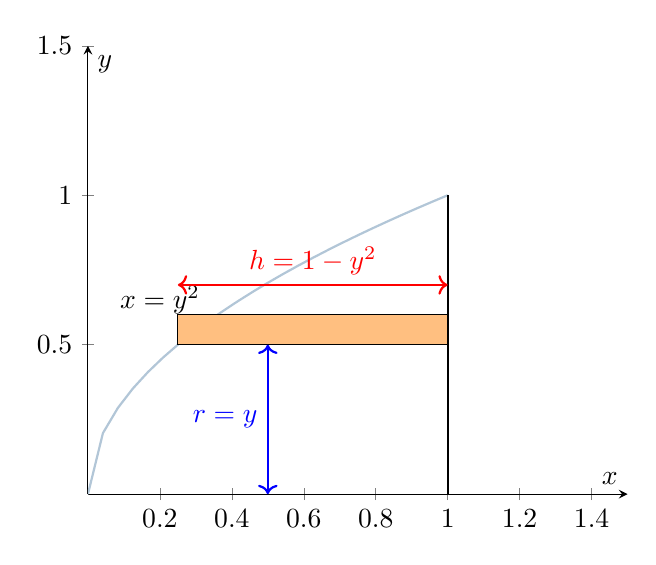
\begin{tikzpicture}
                \begin{axis}[axis lines=middle, xmin=0, xmax=1.5, ymin=0, ymax=1.5, xlabel=$x$, ylabel=$y$]
                    \addplot[thick, UETBlue!30, domain=0:1] {sqrt(x)};
                    \draw[thick] (axis cs:1,0) -- (axis cs:1,1);
                    \draw[fill=orange!50] (axis cs:0.25, 0.5) rectangle (axis cs:1, 0.6);
                    \node at (axis cs:0.2, 0.65) {$x=y^2$};
                    
                    \draw[<->, blue, thick] (axis cs:0.5, 0) -- (axis cs:0.5, 0.5) node[midway, left] {$r=y$};
                    \draw[<->, red, thick] (axis cs:0.25, 0.7) -- (axis cs:1, 0.7) node[midway, above] {$h=1-y^2$};
                \end{axis}
            \end{tikzpicture}
        }
    \end{columns}
\end{frame}

% Slide 7: Ví dụ 3 - Bước 3
\begin{frame}{Ví dụ 3: Quay quanh trục hoành (Vỏ ngang) - Bước 3}
    \textbf{Tính tích phân:}
    \[ V = \int_{0}^{1} 2\pi r(y) h(y) \, dy \]
    
    \pause % Dừng lại để sinh viên tự thay số
    Thay $r=y$ và $h=1-y^2$:
    \begin{align*}
        V &= \int_{0}^{1} 2\pi y (1 - y^2) \, dy \\
          &= 2\pi \int_{0}^{1} (y - y^3) \, dy \\
          \onslide<3->{&= 2\pi \left[ \frac{y^2}{2} - \frac{y^4}{4} \right]_0^1 \\
          &= 2\pi \left(\frac{1}{2} - \frac{1}{4}\right) = 2\pi \cdot \frac{1}{4} = \frac{\pi}{2}}
    \end{align*}
\end{frame}

% Slide 8: Ví dụ 4 - Bước 1
\begin{frame}{Ví dụ 4: Trục quay dịch chuyển ($x=2$) - Bước 1}
    \textbf{Đề bài:} Quay miền $y = x - x^2$ quanh đường thẳng $x=2$.
    \begin{columns}
        \column{0.6\textwidth}
        \textbf{Phân tích:}
        \begin{itemize}[<+->]
            \item Trục quay đứng ($x=2$) song song $Oy \Rightarrow dx$.
            \item \textbf{Bán kính ($r$):} Khoảng cách từ lát cắt $x$ đến trục quay $x=2$.
            \[ r = 2 - x \quad (\text{vì } x < 2) \]
            \item \textbf{Chiều cao ($h$):} Parabol cao $y$.
            \[ h = x - x^2 \]
        \end{itemize}

        \column{0.4\textwidth}
        \centering
        \resizebox{0.9\linewidth}{!}{
            \begin{tikzpicture}
                \begin{axis}[axis lines=middle, xmin=-0.5, xmax=2.5, ymin=-0.5, ymax=1, xlabel=$x$, ylabel=$y$, ticks=none]
                    \addplot[thick, UETBlue!30, domain=0:1] {x - x^2};
                    \draw[dashed, red, thick] (axis cs:2, -0.5) -- (axis cs:2, 1);
                    \draw[fill=orange!50] (axis cs:0.4, 0) rectangle (axis cs:0.45, 0.24);
                    
                    % Dim Radius
                    \draw[<->, blue, thick] (axis cs:0.425, 0.12) -- (axis cs:2, 0.12); 
                    \node[blue, fill=white] at (axis cs:1.2, 0.12) {\tiny $r=2-x$};
                \end{axis}
            \end{tikzpicture}
        }
    \end{columns}
\end{frame}

% Slide 9: Ví dụ 4 - Bước 2
\begin{frame}{Ví dụ 4: Trục quay dịch chuyển ($x=2$) - Bước 2}
    \textbf{Tính toán:}
    \pause
    \begin{align*}
        V &= \int_{0}^{1} 2\pi (2-x)(x-x^2) \, dx \\
          &= 2\pi \int_{0}^{1} (2x - 2x^2 - x^2 + x^3) \, dx \\
          &= 2\pi \int_{0}^{1} (x^3 - 3x^2 + 2x) \, dx \\
          \onslide<3->{&= 2\pi \left[ \frac{x^4}{4} - x^3 + x^2 \right]_0^1 \\
          &= 2\pi \left( \frac{1}{4} - 1 + 1 \right) = \frac{\pi}{2}}
    \end{align*}
\end{frame}

% Slide 10: Tổng kết
\begin{frame}{Tóm tắt Chiến lược Giải bài toán}
    \begin{enumerate}[<+->]
        \item \textbf{Vẽ miền và trục quay:} Xác định tương quan vị trí.
        \item \textbf{Chọn biến tích phân:}
        \begin{itemize}
            \item Trục quay $\parallel Oy \Rightarrow dx$.
            \item Trục quay $\parallel Ox \Rightarrow dy$.
        \end{itemize}
        \item \textbf{Xác định $r$ và $h$:}
        \begin{itemize}
            \item $r$: Khoảng cách từ biến ($x$ hoặc $y$) đến trục quay.
            \item $h$: Độ dài đoạn cắt (Trên - Dưới hoặc Phải - Trái).
        \end{itemize}
        \item \textbf{Công thức:} $V = 2\pi \int r \cdot h \, d(\dots)$
    \end{enumerate}
\end{frame}

% =========================================================
% PHẦN BỔ SUNG
% =========================================================
\section{Phần Bổ sung (Mở rộng)}

% Slide 14: Midpoint
\begin{frame}{Góc nhìn Trực quan - Tổng Riemann Giữa}
    \begin{columns}
        \column{0.55\textwidth}
        \small
        Trong định nghĩa tích phân, việc chọn điểm mẫu $x_i^*$ rất quan trọng.
        \begin{itemize}[<+->]
            \item \textbf{Vấn đề:} Chọn cạnh trái/phải sẽ gây ra "xấp xỉ thừa/thiếu" rõ rệt.
            \item \textbf{Giải pháp (Midpoint):} Chọn điểm giữa $x_i^*$.
            \item \textbf{Ý nghĩa:} Hình chữ nhật \textbf{cắt ngang} đường cong.
            \begin{itemize}
                \item Một phần thừa ra ngoài (màu đỏ).
                \item Một phần thiếu bên trong (màu xanh).
                \item \textbf{Kết luận:} Hai phần này triệt tiêu nhau $\Rightarrow$ Tổng hội tụ nhanh về giá trị thực.
            \end{itemize}
        \end{itemize}

        \column{0.45\textwidth}
        \centering
        % Code hình vẫn giữ nguyên
        \resizebox{0.9\linewidth}{!}{
            \begin{tikzpicture}
                \begin{axis}[
                    axis lines=middle,
                    xmin=0.5, xmax=3.5, ymin=0, ymax=5,
                    xlabel=$x$, ylabel=$y$,
                    ticks=none,
                    height=6cm, width=7cm
                ]
                    \addplot[thick, name path=curve, UETBlue, domain=1:3, smooth] {0.5*(x-1)^2 + 2};
                    \def\xA{1.5} \def\xB{2.5} \def\midX{2} \def\midY{2.5} 
                    \draw[fill=orange!10, thick] (axis cs:\xA, 0) rectangle (axis cs:\xB, \midY);
                    \fill[red] (axis cs:\midX, \midY) circle (2pt) node[above right] {$f(x_i^*)$};
                    \draw[dashed] (axis cs:\midX, 0) -- (axis cs:\midX, \midY);
                    \path[name path=rectTop] (axis cs:\xA, \midY) -- (axis cs:\midX, \midY);
                    \addplot[red!60] fill between[of=rectTop and curve, soft clip={domain=\xA:\midX}];
                    \path[name path=rectTopRight] (axis cs:\midX, \midY) -- (axis cs:\xB, \midY);
                    \addplot[green!60!black] fill between[of=curve and rectTopRight, soft clip={domain=\midX:\xB}];
                    \node[red, font=\tiny] at (axis cs:1.4, 2.7) {Thừa};
                    \node[green!60!black, font=\tiny] at (axis cs:2.6, 2.7) {Thiếu};
                    \draw[<->] (axis cs:\xA, -0.3) -- (axis cs:\xB, -0.3) node[midway, below] {$\Delta x$};
                \end{axis}
            \end{tikzpicture}
        }
    \end{columns}
\end{frame}

% Slide 15: Giải mã ký hiệu Leibniz
\begin{frame}{Giải mã ký hiệu - Sự tương đồng thú vị}
    \begin{columns}
        \column{0.65\textwidth}
        Gottfried Wilhelm Leibniz (người sáng tạo ra ký hiệu này) đã thiết kế nó để gợi nhớ trực tiếp về Tổng Riemann:
        \vspace{1em}
        % [HIỆU ỨNG] Xuất hiện lần lượt 1->2->3
        \begin{enumerate}
            \item<1-> \textbf{Dấu $\displaystyle \int$}: 
            Thực chất là chữ \textbf{S} kéo dài, viết tắt của \textbf{Summa} (tiếng Latin nghĩa là Tổng). Nó tương ứng với dấu xích-ma $\sum$.
            
            \item<2-> \textbf{$f(x)$}: 
            Tương ứng với chiều cao $f(x_i^*)$ của thanh chữ nhật trong tổng Riemann.
            
            \item<3-> \textbf{$dx$}: 
            Tương ứng với chiều rộng $\Delta x$, nhưng mang ý nghĩa là một phần tử "vô cùng bé" (vi phân).
        \end{enumerate}

        \column{0.35\textwidth}
        \centering
        \begin{tikzpicture}
            \node[scale=5, UETBlue] at (0,2) {$\int$};
            \node[scale=3] at (0,0) {$\approx \sum$};
            % [HIỆU ỨNG] Các chú thích cũng hiện ra đồng bộ với text bên trái
            \onslide<1->{\node[anchor=west] at (1,2.5) {\textbf{Summa}};
            \node[anchor=west, gray] at (1,2) {(Tổng)};}
            \onslide<1->{\node[anchor=west] at (1,0.5) {\textbf{Sigma}};}
            
            \draw[->, thick, orange] (0, 0.8) -- (0, 1.2);
            \node[font=\tiny, align=center] at (0, 1) [right] {Liên tục hóa};
        \end{tikzpicture}
    \end{columns}
\end{frame}

\begin{frame}
    \transdissolve % Hiệu ứng tan biến kết thúc
    \centering \Huge \textbf{Cảm ơn Thầy và các bạn!}
\end{frame}

\end{document}

